%导数

% 未完成: 举几个例子,说明常数导数为零, 直线导数为定值等!
\pentry{极限\upref{Lim}}

\subsection{导数的几何理解}

一个一元函数 $y = f\left( x \right)$, 在直角坐标系中表示为一条曲线.在这个曲线的光滑部分取一点 $A$, 并作其切线\upref{TanL}.

\begin{figure}[ht]
\centering
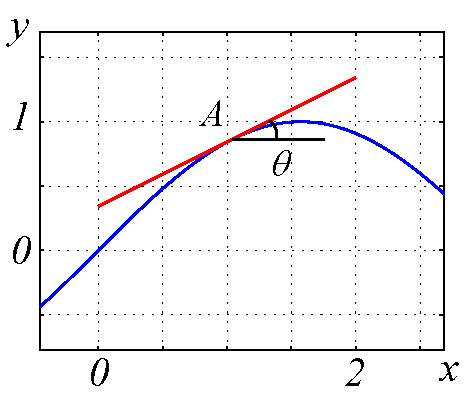
\includegraphics[width=5cm]{./figures/Der1.pdf}
\caption{点 $A$ 的切线}
\end{figure}


若切线存在,该切线与 $x$ 轴的夹角 的正切值 $\theta$ 就叫点 $A$ 的导数.当函数在 $A$ 点递增时,可能的取值为 $\theta  \in \left( {0,\pi/2} \right)$, 即 $\tan \theta  \in \left( {0, + \infty } \right)$. 递减时,取 $\theta  \in (-\pi/2,0)$, 即 $\tan \theta  \in (-\infty ,0)$. 当切线水平时,$\theta  = \tan \theta  = 0$. 

若函数曲线在 $x$ 的某一开区间每一点都可导,则这个区间上每一个 $x$ 对应一个导数.将其写成关于 $x$ 的函数 $g\left( x \right)$,  $g\left( x \right)$  就是该区间上的 \textbf{导函数}. 通常将导函数记为以下的一种(后3种记号的来源见下文)

\begin{equation}\label{Der_eq1}
f'(x),\quad [f(x)]',\quad \dv{y}{x},\quad \dv{f}{x},\quad \dv{x}f(x)
\end{equation}


另外,若切线不存在(例如折线的棱角处,但也有其他更复杂的情况), 我们说点 $A$ 不可导.

\begin{figure}[ht]
\centering
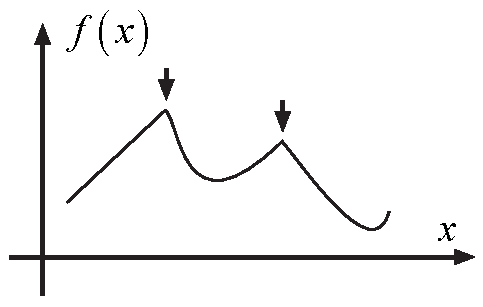
\includegraphics[width=5cm]{./figures/Der3.pdf}
\caption{棱角处不可导}
\end{figure}


若函数曲线在某一点附近是光滑的,那么在这点附近取一小段,当这一段取得足够小,可以近似认为它是线段且与切线重合(如下图). 以这条线段为斜边,作一直角三角形,令其底边长为 $\D x$ (在微积分中,通常把非常小的一段 $\Delta x$ 记为 $\D x$,  $\D x$ 是一不能分割的整体符号,而不是两个量相乘),竖直边的边长为 $\D y$ (当函数递增时, $\D y$ 取正值,反之取负值).根据上面导数的定义,$\dv*{y}{x} = \tan \theta $ 就是函数的导数.所以导数通常表示为 $\dv*{y}{x}$, 导数的倒数则为 $\dv*{x}{y}$. 

\begin{figure}[ht]
\centering
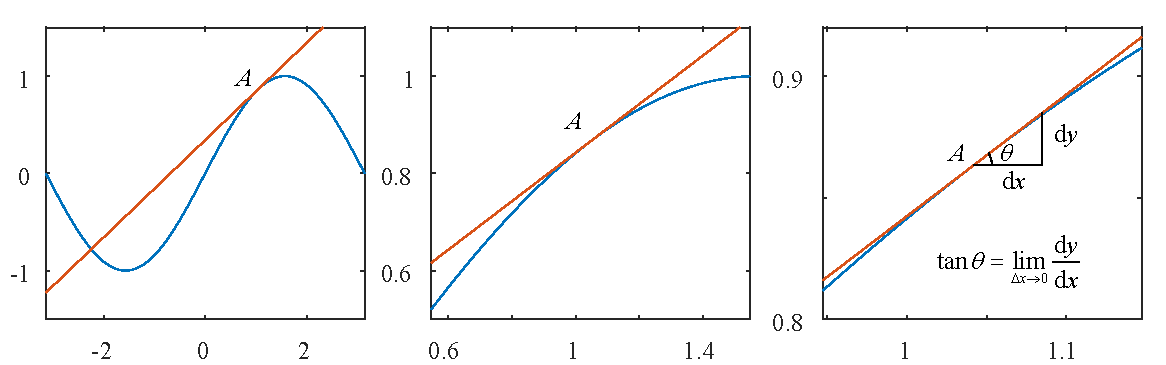
\includegraphics[width=14cm]{./figures/Der2.pdf}
\caption{将切点放大,会发现切线和曲线在切点附近“重合”}
\end{figure}

由上面的讨论可得,当 $x$ 增加一小段 $\Delta x$ 时,$y$ 轴的增量约为 $\Delta y \approx f'\left( x \right)\Delta x$,且当 $\Delta x$ 越小,这条式子就越精确成立, 记为 $\D y = f'(x)\D x$.这个关系就叫函数的微分(看到这里,你可能会觉得,原来微分这么简单! 其实“微积分”基本就是在讲“微分”和“积分” 而一元函数的微分及其基本原理的几何理解基本上就可以认为是上面这张图所表示的).


\subsection{导数的代数理解}

导数的代数理解就是: 一个量关于另一个量的变化率. 例如质点直线运动时,速度的大小就是其路程对时间的导数.把这种描述用极限\upref{Lim}表达出来就是
\begin{equation}\label{Der_eq2}
f'\left( x \right) = \mathop {\lim }\limits_{\Delta x \to 0} \frac{f\left( {x + \Delta x} \right) - f\left( x \right)}{\Delta x}
\end{equation}
在图3的右图中,$\Delta x$ 的始末位置并不非常重要,既可以从 $x$ 取到 $x + \Delta x$, 也可以从 $x - \Delta x$  取到 $x$ 等等( 因为当 $\Delta x$ 非常小的时候,$x$ 附近的曲线基本处处跟切线重合,它们的斜率都是一样的). 所以导数的定义也有其他类似的形式

\begin{equation}
f'\left( x \right) = \mathop {\lim }\limits_{\Delta x \to 0} \frac{f\left( x \right) - f\left( {x - \Delta x} \right)}{\Delta x} = \mathop {\lim }\limits_{\Delta x \to 0} \frac{f\left( {x + \Delta x} \right) - f\left( {x - \Delta x} \right)}{2\Delta x}
\end{equation}
虽然上面用到了诸如“近似”等词,但根据定义,极限都是精确的.


\eentry{一维运动的速度定义,一维运动的加速度定义}

\rentry{基本初等函数的导数\upref{FunDer},求导法则,高阶导数 }%未完成:链接